
%(BEGIN_QUESTION)
% Copyright 2010, Tony R. Kuphaldt, released under the Creative Commons Attribution License (v 1.0)
% This means you may do almost anything with this work of mine, so long as you give me proper credit

Suppose we have an Allen-Bradley SLC 500 PLC connected to two process switches as shown in this illustration:

$$\includegraphics[width=15.5cm]{i04687x01.eps}$$

Determine the bit statuses of {\tt I:1/3} and {\tt I:1/5} when the level switch senses 3 feet and the pressure switch senses 14 PSI.

\underbar{file i04687}
%(END_QUESTION)





%(BEGIN_ANSWER)

Bit statuses:

\begin{itemize}
\item{} {\tt I:1/3} = 1
\item{} {\tt I:1/5} = 0
\end{itemize}

%(END_ANSWER)





%(BEGIN_NOTES)


%INDEX% PLC, relating I/O status to virtual elements 

%(END_NOTES)


